The Standard Model is arguably the most successful theory in all of physics.
It is the culmination of centuries, if not millennia, of scientific advancements and stands as humanity's best answer to the age-old question---what is everything made of, what are the rules governing it?
The Standard Model is formulated in the language of quantum field theory (QFT) and describes the elementary particles and their interactions via the electromagnetic, weak, and strong forces.
When including massive neutrinos in the standard model, it contains 26 free parameters.
These are quantities, such as the masses of particles and the strength of the forces, which cannot be calculated using the Standard Model but must be measured and put in by hand.
This might seem like a lot of freedom, but it is a vanishing amount when compared to the Standard Model's vast amount of precise prediction~\cite{Schwartz:QFT,griffiths:introduction,kramer:the_standard_model}.
\autoref{fig:the standard model} illustrates the particles in the Standard Model.

\begin{figure}[h]
    \centering
    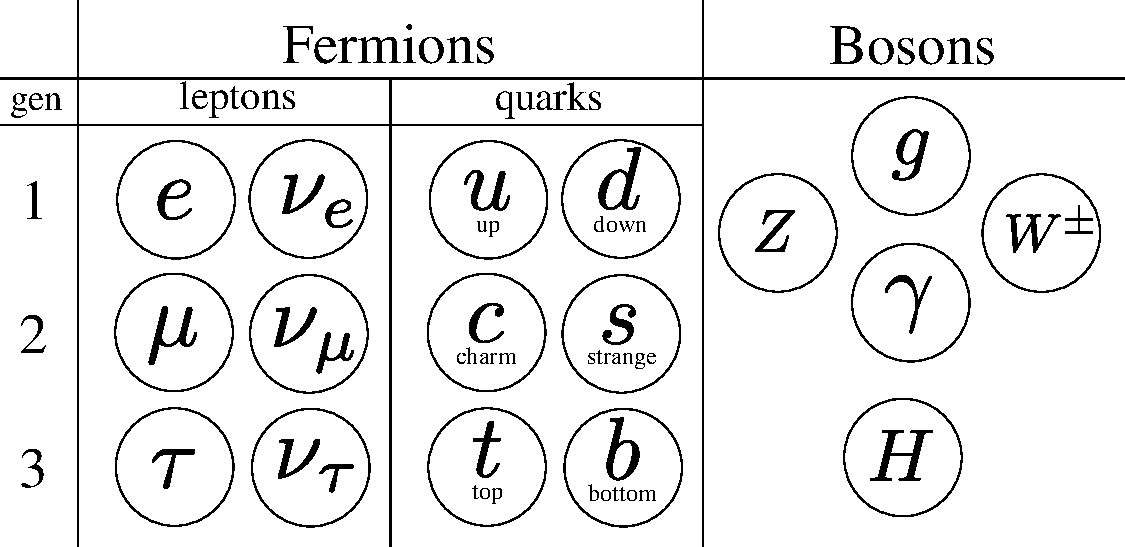
\includegraphics[width=0.7\textwidth]{figurer/standard_model2.pdf}
    \caption{The particles of the Standard Model. The fermions are made up of two leptons and two quarks in each generation, with three generations. The photon ($\gamma$) is the particle of the electromagnetic force, the gluon (g) of the strong force, and the $Z$ and $W^\pm$ bosons are responsible for the weak force. The final piece of the puzzle is the Higgs boson (H).}
    \label{fig:the standard model}
\end{figure}

When we use quantum electrodynamics (QED), the quantum theory of electromagnetic interactions, and the theory of weak interactions to calculate observable quantities, we get highly precise predictions that agree with experiments to an astounding degree~\cite{Schwartz:QFT}.
These calculations are done using perturbation theory.
Perturbation theory is a calculation scheme available for weakly coupled interactions.
It describes a process as the sum of all possible sequences of interactions that could give rise to that process.
A Feynman diagram illustrates each such possible sequence.
Together with the Feynman rules, each Feynman diagram is a recipe for calculating the contribution of that particular sequence to the total sum.
\autoref{fig:qed feynman diagrams} illustrates the lowest order contributions to the process of electron-electron scattering.
The weakness of QED is quantified in the fine structure constant, $\alpha \approx 0.00 7297$~\cite{PDG}, one of the free parameters mentioned earlier.
Each vertex in a QED Feynman diagram is proportional to $\alpha$.
A diagram with $n$ vertices is proportional to $\alpha^n$.
This tends to zero as $n$ approaches infinity, and as a result, a complicated Feynman diagram---with many vertices and thus also many loops---will generally give a small contribution to the overall sum.
In the case of QED, calculating a few orders in perturbation theory yield precise and accurate estimates.\footnote{The magnitude of a complicated diagram is small, but there are also a lot of them. The inclusion of higher-order diagrams will eventually lead to large corrections, and the sum will diverge~\cite{dyson:divergence_of_perturbation}. In QED, this is estimated to occur for diagrams of order $n \approx 1 / \alpha \approx 137$, which is far more than we could hope to calculate at present. Perturbation theory must be interpreted, not as a convergent series, but an asymptotic expansion, which gives accurate estimates when truncated~\cite{flory:how_i_learn_to_stop}.}

\begin{figure}[h]
    \centering
    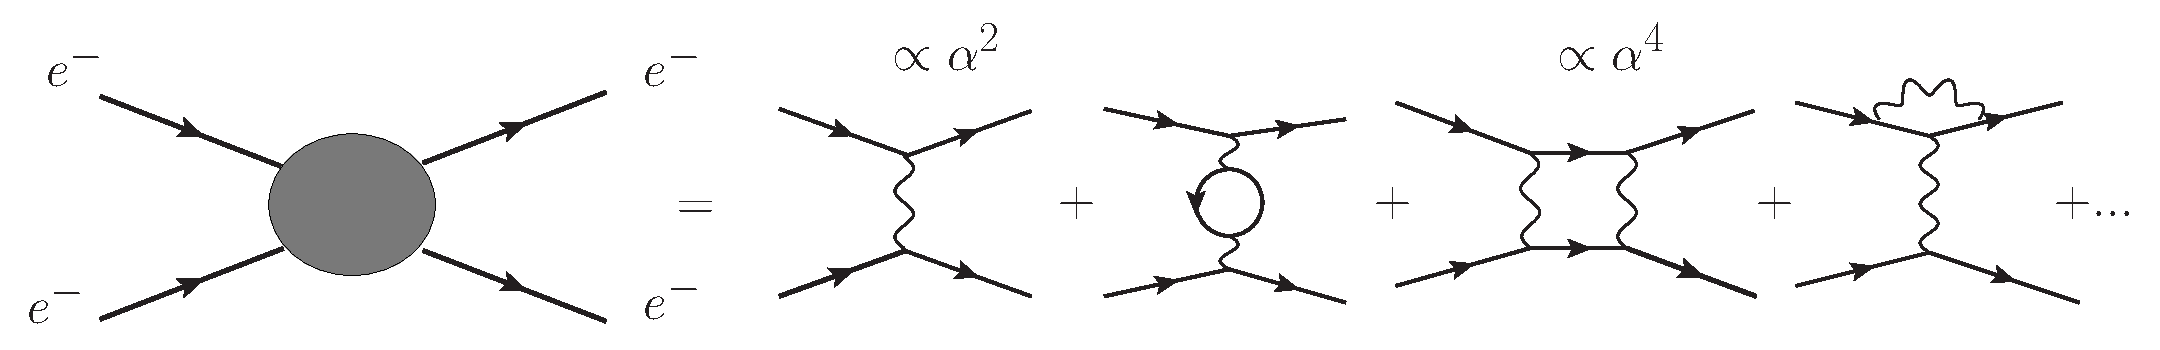
\includegraphics[width=0.95\textwidth]{figurer/feynman-diagram/sum_qed.eps}
    \caption{The process of electron-electron scattering is described by the summation of Feynman diagramms representing all possible ways for the electrons to interact. Higher order terms are less important, as they pick up more and more powers of $\alpha$. Diagrams are drawn using~\cite{JaxoDraw}.}
    \label{fig:qed feynman diagrams}
\end{figure}

Quantum chromodynamics, or QCD, is the part of the Standard Model that describes quarks, the constituents of protons and neutrons, and how they interact via the strong nuclear force.
When dealing with the strong force, the fact that the strength of interaction depends on the energy scale becomes apparent.
This dependence is due to what is called the \emph{running} of the coupling constant.
In high energy interactions at the energy scale of the $Z$-boson, $m_z \approx 91.19 \, \text{GeV}$, the strong force equivalent to the fine structure constant is $\alpha_s(m_Z) \approx 0.118$~\cite{PDG}.
This makes it possible to do perturbative calculations using QCD.
However, the strong force has its name for a reason.
For scales around $1\, \text{GeV}$ and below, the perturbation method breaks down.
In this case, quarks bond together and form \emph{hadrons}.
Hadrons are classified as \emph{mesons} or \emph{baryons}.
The most familiar of the baryons are the proton and neutrons.

None of the mesons are stable, but they play an essential role in describing the strong force in the non-perturbative regime.
This is done using \emph{effective field theories}, which we will cover in the following subsection.
Mesons, of which pions are the lightest, were first proposed by Hideki Yukawa as the mechanism to hold nucleons together and form the nucleus of atoms.
Though first believed to appear in the showers of particles created by cosmic rays, they were decisively discovered in 1947 by Cecil F. Powell \emph{et al.}~\cite{griffiths:introduction}.
Pions do not show up in the standard model, as quarks do, but rather as an effective degree of freedom at low energy.


\subsection*{Effective field theories}

A profound feature of physics is the possibility of describing a system by isolating the degrees of freedom of interest, ignoring the rest.
We can describe the motion of the planets in the solar system, massive and complex systems, by only their mass, velocity, and position.
In quantum field theory, this feature manifests in the power of effective field theory.
An effective field theory describes a system not by the fundamental, underlying particles but by effective degrees of freedom.
A theory of two interacting fields $\varphi$ and $\psi$ will be described by an action that depends on both fields, $S[\varphi, \psi]$.
In the path integral formalism, predictions can then be made by integrating over all possible states of the fields.
An example is the vacuum transition amplitude,
\begin{equation}
    Z = \int \D \varphi \D \psi \, \exp{i S[\varphi, \psi]}.
\end{equation}
We obtain an effective description of only the $\varphi$-degrees of freedom by \emph{integrating out} the $\psi$-degrees of freedom, which results in an effective action $S_\text{eff}[\varphi]$, related to the underlying theory by~\cite{Schwartz:QFT}
\begin{equation}
    \label{integrating out degrees of freedom}
    \int D \varphi \, \exp{i S_\text{eff}[\varphi]}
    =
    \int \D \varphi \D \psi \, \exp{i S[\varphi, \psi]}.
\end{equation}
This gives us hope for describing low-energy QCD as an effective theory of the particles we observe in experiments.
In this specialization project, we will derive and explore chiral perturbation theory (\chpt), a low-energy effective theory of QCD where mesons are the degrees of freedom.

The action of the standard model has the form of an integral over a local Lagrangian,
\begin{equation}
    S[\varphi] = \int \dd^4 x \, \Ell[\varphi],
\end{equation}
where $\varphi$ denotes all fundamental particles.
The locality of $\Ell$ means that it is made up of terms like $\varphi(x) \varphi(x)$, where all interactions happen at one point in space-time, as opposed to a term such as $f(x, y)\varphi(x) \varphi(y)$.
We can not a priori expect an effective action to take this form~\cite{Schwartz:QFT}.
However, we have general principles we expect particles to obey, such Lorentz invariance and cluster decomposition.
Cluster decomposition concerns a system of $N$ sets of particles, $\alpha_i$, that evolve into the sets $\beta_i$.
That is,
\begin{equation}
    \ket{\alpha_1, \alpha_2, ... \alpha_N}_\text{in}
    \longrightarrow
    \ket{\beta_1, \beta_2, ... \beta_N}_\text{out}.
\end{equation}
It says that if the sets of particles $\alpha_i$, $\beta_i$ are located far enough apart, then the $S$-matrix factors as
\begin{equation}
    {\braket{\beta_1, \beta_2, ... \beta_N}{\alpha_1, \alpha_2, ... \alpha_N}}
    =
    \braket{\beta_1}{\alpha_1}\braket{\beta_2}{\alpha_2}... \braket{\beta_N}{\alpha_N}.
\end{equation}
This is a familiar property, as it essentially says that wildly separated experiments do not interfere, and one that we expect all good effective descriptions to have~\cite{weinberg_1995,weinberg_1996_vol2}.
These principles greatly constrain any effective action and are the basis for constructing the \chpt\, effective action.
This method was formulated by Weinberg~\cite{WeinbergPhenom}
It relies on---as Weinberg himself called it---a ``theorem'':
\begin{quote}
    ``[I]f one writes down the most general possible Lagrangian, including all terms consistent with assumed symmetry principles, and then calculates matrix elements with this Lagrangian to any given order of perturbation theory, the result will simply be the most general possible $S$-matrix consistent with analyticity, perturbative unitary, cluster decomposition and the assumed symmetry principles.'' \cite{WeinbergPhenom}
\end{quote}
In other words, if we write down the most general Lagrangian consistent with symmetries of the underlying theory, then we have not made any restrictions on the theory, other than some foundational assumptions.
This Lagrangian will be of the form
\begin{equation}
    \Ell_\text{eff}[\varphi] = \sum_i \lambda_i \mathcal O_i,
\end{equation}
where $\mathcal O_i$ are local functions of the fields and their derivatives, and $\lambda_i$ are coupling constants.
The coupling constants are free parameters, which parametrizes the most general $S$-matrix consistent with foundational assumptions and the underlying theory.
A Lagrangian with an infinite amount of free parameters might seem useless.
However, if we can find a consistent series expansion, then only a finite number of terms are needed to calculate quantities to any given order in perturbation theory.
In the case of \chpt, the expansion is in the momentum of the pions.
We will detail this later in the text.


\subsection*{Stars}

Although it might seem counterintuitive, stars are one of the objects we might hope to describe using QCD at low energies.
Neutron stars, one of the most extreme objects in the universe, quickly cool down to temperatures below $10^{10} \, \text{K}$.
This might be hot by almost all standards.
However it corresponds to an energy of $0.862 \, \text{MeV}$.
This is well below the perturbative regime of QCD, and the stars must therefore be described by an effective model of interacting nuclear matter~\cite{glendenning:compcat_stars,from_hadrons_to_quarks}.
Stars are modeled using the Tolman-Oppenheimer-Volkoff, or TOV, equations.
The TOV equations are based on Einstein's general theory of relativity, and its solution gives the star's pressure as a function of its radius.
The only input needed is the \emph{equation of state}, or EOS, of the matter that makes up the star~\cite{Carroll:space-time}.
The equation of state of a system is the relationship between its energy density, $u$, and pressure $P$, i.e. a relationship of the form
\begin{equation}
    f(P, u) = 0.
\end{equation}
This is where QCD comes in.
One way to compute the equation of state of QCD systems is using the numerical method called lattice QCD.
Here, space-time is approximated as finite and discrete, and Monte-Carlo importance sampling is used to perform the path integral.
This method, however, fails for non-zero baryon chemical potential $\mu_B$, in what is known as the fermion sign problem.
The baryon chemical potential $\mu_B$ parametrizes the matter-antimatter asymmetry.
A high value of $\mu_B$ corresponds to a high matter density.
There is much more matter than antimatter in neutron stars, or more generally, all observed stars.
This makes lattice QCD unsuited for simulating these systems.
Recently, pions have been proposed to form a new type of compact, gravitationally bound object, i.e., a star.
Pions can form states with zero baryon chemical potential, which are thus amenable to lattice QCD simulations.
This offers a way to model stellar objects from first principles, as well as by analytical methods using \chpt~\cite{new_clas_of_compact_stars,andersen:bose_einstein}.

\subsection*{Pion condensate and the QCD phase diagram}

In addition to their electrical charge, pions have an \emph{isospin} quantum number, $I_3 = -1, 0$ or $1$, and a corresponding isospin chemical potential $\mu_I$.
This chemical potential parametrizes how much the system favors negative or positive isospin charges.
When the isospin chemical potential reaches a critical value, $\mu_I = \mu_I^c$, the system undergoes a phase transition and form a pion condensate with a non-zero isospin density $n_I$.
The pion condensate is an expample of Bose-Einstein condensation, in which a macroscopic number of bosons occupy a single quantum state~\cite{Brandt:QCD_phase_diagram_with_isospin_chemical_potential,Brandt:QCD_phase_diagram_for_nonzero_isospin-asymmetry,mannarelli:meson_condensation}.

\begin{figure}[ht]
    \centering
    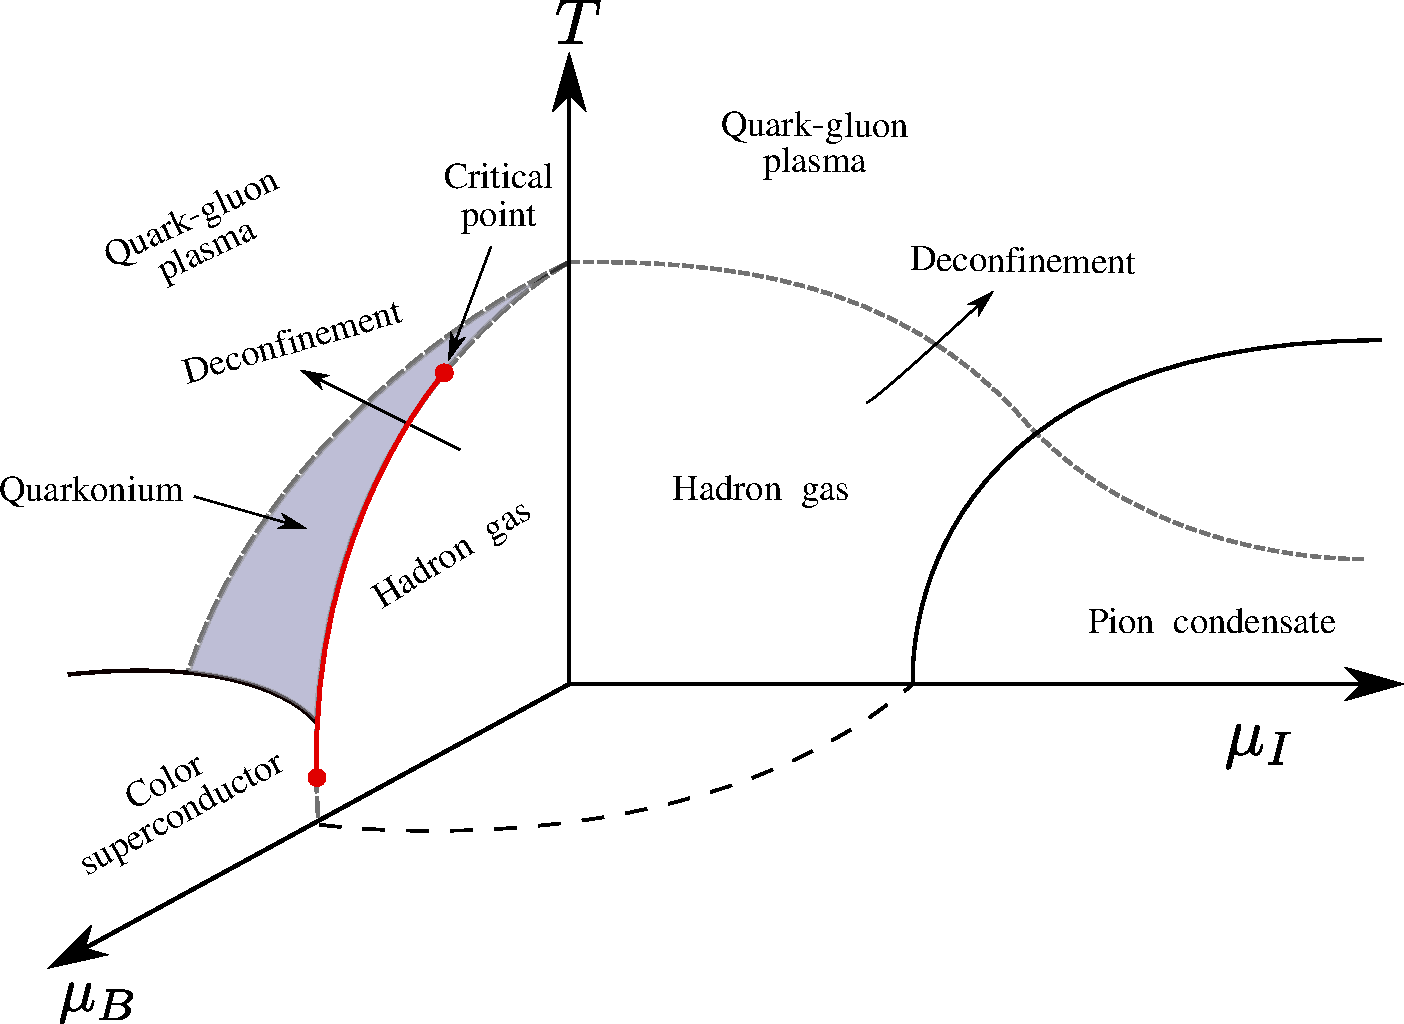
\includegraphics[width=\textwidth]{figurer/phase_diagram2.pdf}
    \caption{A sketch scetch of the phase diagram of QCD. See text for description. Based on~\cite{from_hadrons_to_quarks,
            Brandt:QCD_phase_diagram_with_isospin_chemical_potential,Brandt:QCD_phase_diagram_for_nonzero_isospin-asymmetry,Fukushima:The_phase_diagram_of_dense_QCD,mannarelli:meson_condensation,alford:color_superconductivity}
    }
    \label{fig:phase diag qcd}
\end{figure}

The pion condensate phase is just one part of the rich phase structure of QCD, which is an active field of research.
In \autoref{fig:phase diag qcd}, we show a rough sketch of this diagram.
We emphasize that the understanding of this diagram is far from complete.
The difficulties of exploring QCD, such as the non-perturbativity at low temperatures and the fermion sign problem mentioned in this text, means that much of the phase diagram is only conjectured.
At low temperatures and chemical potentials, where the strong interaction is just that, strong, QCD-matter form a hadronic gas.
This is called the normal phase or vacuum phase.
Here, QCD is best described by an effective theory of hadrons.
QCD matter is in its vacuum phase in all but the most extreme situations.
In the case where the hadronic description fails, under extreme temperatures or densities, \emph{quark matter} is formed.
Quark matter is conjectured to be present at the center of neutron stars~\cite{from_hadrons_to_quarks}, and there were done observations of a non-hadronic state of QCD-matter at the Relativistic Heavy Ion Collider (RHIC) in 2005~\cite{2005:RHIC,2005:RHIC2}.

At high temperatures, QCD-matter undergoes \emph{deconfinment}, as the strong force weakens due to the running of the coupling constant.
In this phase, quarks are no longer tightly bound in hadrons, but together with gluons form a soup called \emph{quark-gluon plasma}.
At $\mu_B = \mu_I = 0$, the crossover from the vacuum phase to a quark-gluon plasma is characterized by the pseudo-critical temperature, $T_{pc}$, which is estimated to be in the range of $150 \, \text{MeV}$ to $200 \, \text{MeV}$~\cite{Fukushima:The_phase_diagram_of_dense_QCD}.
At low temperatures and high baryon density, and thus high $\mu_B$, the hadron gas undergoes a liquid-gas phase transition.
This happens when $\mu_B \approx m_N = 939 \, \text{MeV}$, where $m_N$ is the neucleon mass~\cite{Fukushima:The_phase_diagram_of_dense_QCD}.
At arbitrarily high $\mu_B$, rigorous results are available which show QCD-matter form a color-superconducting phase.
The color-superconductor is a state of matter analogous to electrical superconductors, in which electrons form Cooper pairs allowing for unimpeded electrical current.
The color superconducting phase is due to Cooper pairs of quarks forming and results in effects such as the Meissner effect in which gluons can acquire mass.
The nature of the transition between cold hadronic matter to a color-superconducting phase is not well understood~\cite{alford:color_superconductivity}.

Understanding the phase diagram of QCD is an integral part of research into the standard model and its consequences.
It is essential to use all possible sound approaches to validate the techniques used.
This allows for validation of methods by comparing results in the overlapping regimes, such as when comparing \chpt\ with lattice QCD.


\subsection*{Outline of thesis}
In this specialization project we calculate the next-to-leading order equation of state of a system at finite isospin chemical potential, using two-flavor chiral perturbation theory.
We will also investigate the phase transition from the vacuum phase into a pion condensate phase.
In \autoref{chapter:theory}, we take a survey of some general theory needed for \chpt.
We introduce the generating functional in the path integral formalism and use this to define the one-particle-irreducible effective action and the effective potential.
This allows us to prove Goldstone's theorem, a significant result that connects the symmetries of a theory to its low energy dynamics.
The theorem states that spontaneous symmetry breaking gives rise to massless particles.
We then present the CCWZ construction, which provides a procedure to construct an effective Lagrangian of Goldstone bosons.
We also present some mathematical prerequisites, such as Lie groups and Lie algebras, and discuss the role and mathematical implementation of symmetries in physics in general and quantum field theory in particular.

In \autoref{chapter:effective theory of pions}, we take the general theory of the last chapter and apply it to QCD.
We start the chapter by discussing QCD, its constituent parts, symmetries, and the corresponding conserved currents.
We then use the theory from the last chapter to find the terms that make up the Lagrangian of \chpt\, and incorporate explicit symmetry breaking, external source currents, and a finite isospin chemical potential.
This section also discusses how to order these terms in a well-defined series expansion.
With this, we construct the leading order and next-to-leading order Lagrangian, which is expanded in powers of the pion fields.
We use our result to find properties of the pion, such as their tree-level mass and propagator.

\autoref{chapter:thermodynamics} is dedicated to the thermodynamic properties of \chpt.
We use the derived Lagrangian to calculate the free energy density to one loop using the leading order Lagrangian.
Then, we use the tree level free energy density at next-to-leading order to renormalize the result.
We discuss the low energy parameters we use and how to consistently evaluate observable to the same order in the series expansion.
With the free energy density, we derive the equation of state at finite isospin chemical potential.
We also discuss the phase transition to the pion condensate phase using the Landau theory of phase transitions.

In \autoref{chpater:conclusion and outlook}, we summarize the results and discuss further work.
The appendix is referenced throughout the text.
In \autoref{appendix:thermal field theory}, we review thermal field theory and the imaginary time formalism.
This chapter contains details of calculations used in the main text, where they are referenced.
We also discuss dimensional regularization, derive the Feynman rules for and interacting scalar, and generalize thermal field theory to fermions.
\autoref{section:algebra bases}, \autoref{section:Functional derivative} and \autoref{appendix:rewriting terms} contain additional material, and are referenced when relevant.
In \autoref{appendix:computer code}, we link to an online repository containing all computer code used in this project.
